LangChain è un framework per lo sviluppo di applicazioni basate su modelli linguistici.

Il framework non si limita ad offrire un'interfaccia per l'uso di modelli linguistici, ma offre anche un'interfaccia per realizzare applicazioni:

\begin{itemize}
    \item Che sappiano utilizzare informazioni che non sono state oggetto del training, tramite database esterni o internet
    \item Che sappiano interagire con gli strumenti che uno sviluppatore gli mette a disposizione
\end{itemize}

Il framework LangChain offre due principali strumenti:

\begin{itemize}
    \item Componenti: LangChain fornisce astrazioni modulari per i componenti necessari a lavorare con i modelli linguistici. LangChain ha anche collezioni di implementazioni per tutte queste astrazioni. I componenti sono progettati per essere facili da usare, indipendentemente dall'utilizzo del resto del framework.
    \item Catene specifiche per i casi d'uso: Le catene possono essere pensate come l'assemblaggio di questi componenti in modi particolari, al fine di realizzare al meglio un particolare caso d'uso. Sono intese come un'interfaccia ad alto livello attraverso la quale si può facilmente iniziare a lavorare con un caso d'uso specifico. Queste catene sono anche progettate per essere personalizzabili.
\end{itemize}

\subsection[I componenti]{I componenti}
I componenti sono i mattoni fondamentali di LangChain.
Sono progettati per essere facili da usare e integrare, indipendentemente dall'utilizzo del resto del framework.
La prima tipologia di componenti che offre LangChain sono gli \textbf{schema}.
\subsubsection*{Schema} Gli schema sono il modo in cui LangChain rappresenta il testo e le interazioni che si possono avere con i modelli.

Negli schema ci sono quattro tipologie di oggetti:
\begin{itemize}
    \item \textbf{Prompts}: I prompts possono essere semplici stringhe o oggetti più complessi. Tra i prompts più utilizzati i \textit{PromptsTemplate} \label{PromptsTemplate}, ossia delle stringhe che possono essere completate da valori dinamici tramite dei placeholder e i \textit{ChatPromtsTemplate} che sono delle chat sotto forma di template. 
    \item \textbf{ChatMassages}: Sono tipologie di messaggi che rappresentano, letteralmente, una chat con un language model. Possono essere composti da 3 tipologie di messaggi: \textit{SystemChatMessage}, messaggi che rappresentano delle informazioni di contesto per il modello; \textit{HumanChatMessage}, i messaggi che un utente ha inviato al modello; \textit{AIChatMessage}, le risposte che il modello ha inviato all'utente.
    \item \textbf{Examples}: Sono esempi di input e output che possono essere utilizzati sia per il training di un modello, come esempi da imparare, che per la valutazione sia del modello che di una chain dopo aver ottenuto il risultato.
    \item \textbf{Documents}: Rappresentano dei documenti che il modello può utilizzare. Possono essere utilizzati per dividere documenti reali in parti, inserirle in un database e poi essere interrogati.
\end{itemize}

Questi Schema sono i mattoni fondamentali con cui si vanno poi ad utilizzare il secondo tipo di componenti: i \textbf{modelli}.

\subsubsection*{Modelli}
I modelli sono gli oggetti con cui il framework LangChain rappresenta i modelli linguistici e le API con cui interagire con essi.

Il framework divide i modelli in due categorie:
\begin{itemize}
    \item \textbf{Modelli di linguaggio}: Sono modelli che hanno come scopo quello di generare testo. Possono essere utilizzati per generare testo a partire da un prompt, per completare un prompt o per generare testo a partire da un documento.
    \item \textbf{Modelli di chat}: Sono modelli che hanno come scopo quello di simulare una conversazione. 
\end{itemize}

I modelli supportati dal framweork possono essere sia derivanti da soluzioni commerciali come quelli di OpenAI, sia modelli sviluppati dalla community opensource se messi su HuggingFace.
Nell'implementazione in python, tutti i modelli vengono utilizzati come funzioni che ricevono in input una stringa.
Per una lista completa delle integrazioni già supportate si può visitare il link \url{https://python.langchain.com/docs/integrations/llms/}.

\subsubsection*{Indici}

Gli indici si riferiscono alle modalità per strutturare i documenti in modo che i modelli di linguaggio di grandi dimensioni possano interagire al meglio con essi.

Per indici si intendono memorie esterne che il language model può interrogare.

Il modulo riguardante gli indici include anche una serie di strumenti per maneggiare i documenti, tra i quali:

\begin{itemize}
    \item \textbf{Document loaders}: Sono classi e funzioni che caricano i documenti da una sorgente esterna, possono essere pdf, file di testo, pagine web oppure personalizzati. La lista completa si trova al link \url{https://python.langchain.com/docs/integrations/document_loaders/}
    \item \textbf{Text splitters}: Sono classi e funzioni che prendono in input un testo (o documento) molto lungo e lo dividono in parti più piccole. La divisione può esser fatta in molti modi, dal banale carattere alla più complessa divisione in frase o paragrafi semanticamente significativi. La divisione in chunk più piccoli è necessaria per prendere i vettori degli embeddings più precisi e quindi facilitare il lavoro dei retriever.
    \item \textbf{Retrievers}: Sono classi che prendono in input un testo e restituiscono un sottoinsieme di documenti che sono rilevanti per il testo in input. I retriever possono essere utilizzati per trovare i documenti che contengono le informazioni necessarie per rispondere a una domanda.
    \item \textbf{Vector stores}: Sono le classi che permettono l'interazione con un database di vettori e la relativa modalità di interrogazione, possono essere utilizzati direttamente oppure tramite un retriever. Ogni database di vettori mette a disposizione una classe che ha firme comuni alle altre e può essere utilizzato in LangChain.
\end{itemize}

Un altro tipo di memorie invece sono ciò che LangChain chiama ``Memory''.

\subsubsection{Memory}
Quando si parla di ``Memory'' in LangChain ci si riferisce alla memoria, o meglio uno stato, della conversazione fin'ora che c'è stata tra l'utente e un modello.

Questo tipo di memoria viene appesa ad ogni input dato all'utente, eventualmente aggiornata, ed è quindi utilizzata per lo più per contenere informazioni di contesto.

I dati che vengono presi da un vector database sono inseriti in questo tipo di memoria per poi esser letti dal modello e utilizzati per generare una risposta.

Essendo una memoria inserita nell'input, consuma token.

Tutti questi elementi sono la base su cui si basano i due componenti più importanti di LangChain: le \textbf{catene} e gli \textbf{agenti}.

\subsubsection*{Catene}

Per ``catena'' si intende un'interfaccia ad alto livello che permette di utilizzare una serie di componenti, modelli (diversi e non) o addirittura altre catene in modo più o meno sequenziale.

Le catene più comuni sono quelle denominate LLMChain, che combinano un \hyperref[PromptsTemplate]{PromptsTemplate} seguito da un modello e eventualmente un parser dell'output per trasformarlo in un formato diverso.

Altra tipologia molto importante di catena, che è anche la tipologia di catena utilizzata per realizzare il lavoro di tesi, è quella che ha a corredo l'interazione con un retriever e quindi con un index.
Questa tipologia di catene, al momento, ha quattro configurazioni principali che si riferiscono a come la catena interagisce con i documenti ricevuti da un retriever:
\begin{itemize}
    \item \textbf{Stuff}: è la tipologia più semplice, in cui si prendono i documenti correlati con l'input dell'utente e li si inserisce nella memoria della conversazione. Ha come principale pro la semplicità dell'utilizzo e il costo, dato che viene fatta una sola chiamata al modello.
    Come contro principale ha il fatto che tutti i LLM hanno una lunghezza massima di input e se i documenti (o chunk di documenti) sono troppo lunghi si potrebbero avere problemi di infattibilità della richiesta. 
    \item \textbf{Map reduce}: proprio come l'algoritmo utilizzato nel mondo hadoop per il calcolo distribuito, questa tipologia di catena esegue la query su ogni documento ricevuto dal retriever e poi aggrega le varie risposte in un unico testo che viene restituita come risposta.
    Questo tipo di catene non ha problemi di scaling, dato che ogni richiesta viene fatta su un singolo documento, ma risulta anche il suo contro principale dato il costo più alto, inoltre è possibile che si perdano informazioni realizzando l'aggregazione.
    \item \textbf{Refine}: l'algoritmo utilizzato è proprio quello di refine, ovvero si prende il primo documento, si fornisce una prima risposta alla query dell'utente e poi ogni documento successivo aggiorna la risposta migliorandola con nuove informazioni derivanti dal nuovo documento.
    Questo tipo di catene ha come pro il fatto che non si perdono informazioni e che il costo è più basso rispetto a map reduce, ma ha come contro il fatto che non è possibile parallelizzare in modo semplice, dato che la risposta deve essere aggiornata sequenzialmente.
    \item \textbf{Map-Rerank}: diversamente dagli altri algoritmi questa tipologia di catene non combina più documenti per dare una singola risposta ma esegue la query su tutti i documenti e fa una classifica della risposta che, secondo il LLM, è più completa. La migliore viene poi restituita come risposta.
    Come costi è simile al refine, ma ha dei casi d'uso diversi dai precedenti, infatti questa tipologia è utilizzabile quando si sa che la risposta migliore è sempre contenuta in un unico documento. 
\end{itemize}

Per la realizzazione della tesi è stata utilizzata la tipologia di catena ``Refine'' poiché i libri trattano per lo più argomenti simili e quindi è possibile che la risposta migliore esca fuori dal miglioramento della prima risposta che si trova.

\subsubsection*{Agenti}

Alcune applicazioni hanno casi d'uso che non possono essere realizzati con una singola catena, ma hanno bisogno di un sistema più complesso e meno lineare.

Per questi casi nascono gli agenti, ovvero una serie di modalità di interrogare un LLM in modo tale che sia lui a decidere i prossimi passi da realizzare all'interno di un ragionamento più ampio.

Langchain offre gli strumenti necessari per implementare gli agenti, nel dettaglio:

\begin{itemize}
    \item \textbf{Agent}: è l'interfaccia che rappresenta un agente, è un wrapper attorno ad un modello che prende in input un testo e restituisce la prossima azione da svolgere.
    \item \textbf{Tool}: sono funzioni che rappresentano delle azioni che un agente può effettuare, questo tipo di azioni possono essere funzioni python anche molto complesse e includere, per esempio, anche chiamate ad altri llm o agenti. Sono il modo in cui un programmatore può iniettare codice all'interno del ragionamento di un modello.
    \item \textbf{Tollkits}: sono aggregazioni di tool. Sono necessari quando i tool sono molti e, dato il limite di token in ingresso dei modelli, si vuole rendere più leggero il contesto.
    \item \textbf{Agent Executor}: sono le classi che mettono insieme i tool e gli agenti, sono loro che realizzano il ragionamento e coordinano le azioni del agent.
\end{itemize}

Gli agenti possono essere di vario tipo che possono performare meglio su alcune tipologie di task rispetto ad altre, per una lista completa si può visitare il link \url{https://python.langchain.com/docs/modules/agents/agent_types/}.

Nel lavoro di tesi non è stato utilizzato un agente ma, sicuramente, in sviluppi futuri si potrebbe pensare di utilizzarne uno per migliorare l'esperienza utente.

\subsection[Chain specifiche]{Le chain ad uso specifico}

Le chain ad uso specifico sono delle catene che sono state realizzate per risolvere un particolare caso d'uso e facilizzare l'esperienza di sviluppo.

Ne esistono di vario tipo, per una lista completa si può visitare il link \url{https://docs.langchain.com/docs/category/use-cases}.

In questo lavoro di tesi ci concentreremo sul caso d'uso del Question Answering Over Docs, ossia una catena pensata e realizzata per rispondere a domande a partire da documenti.

\subsubsection[QA Over Docs]{Question Answering Over Docs}

La procedura per convertire dati grezzi e non strutturati in una catena di domande e risposte (Question Answering) si presenta nel seguente modo (figura~\ref{fig:qaoverdocs}):

\begin{enumerate}
    \item \textbf{Fase di Caricamento}: Inizialmente è necessario caricare i dati. I dati non strutturati possono essere prelevati da diverse fonti. Utilizziamo l'integrazione con LangChain per esplorare l'insieme completo di strumenti di caricamento. Ciascuno di questi strumenti restituisce i dati sotto forma di un Documento LangChain.
    \item \textbf{Fase di Suddivisione}: Gli strumenti di suddivisione del testo frammentano i Documenti in parti di dimensioni specificate.
    \item \textbf{Fase di Archiviazione}: L'archiviazione (ad esempio, spesso tramite un vectorstore) conterrà e spesso incorporerà le parti precedentemente suddivise.
    \item \textbf{Fase di Recupero}: L'applicazione recupera le parti precedentemente archiviate (spesso utilizzando incorporamenti simili a quelli della domanda in ingresso).
    \item \textbf{Fase di Generazione}: Un Linguaggio Modello di Grande Dimensione (LLM) produce una risposta utilizzando uno stimolo che include la domanda stessa e i dati recuperati precedentemente.
\end{enumerate}

\begin{center}
    \begin{figure}[H]
        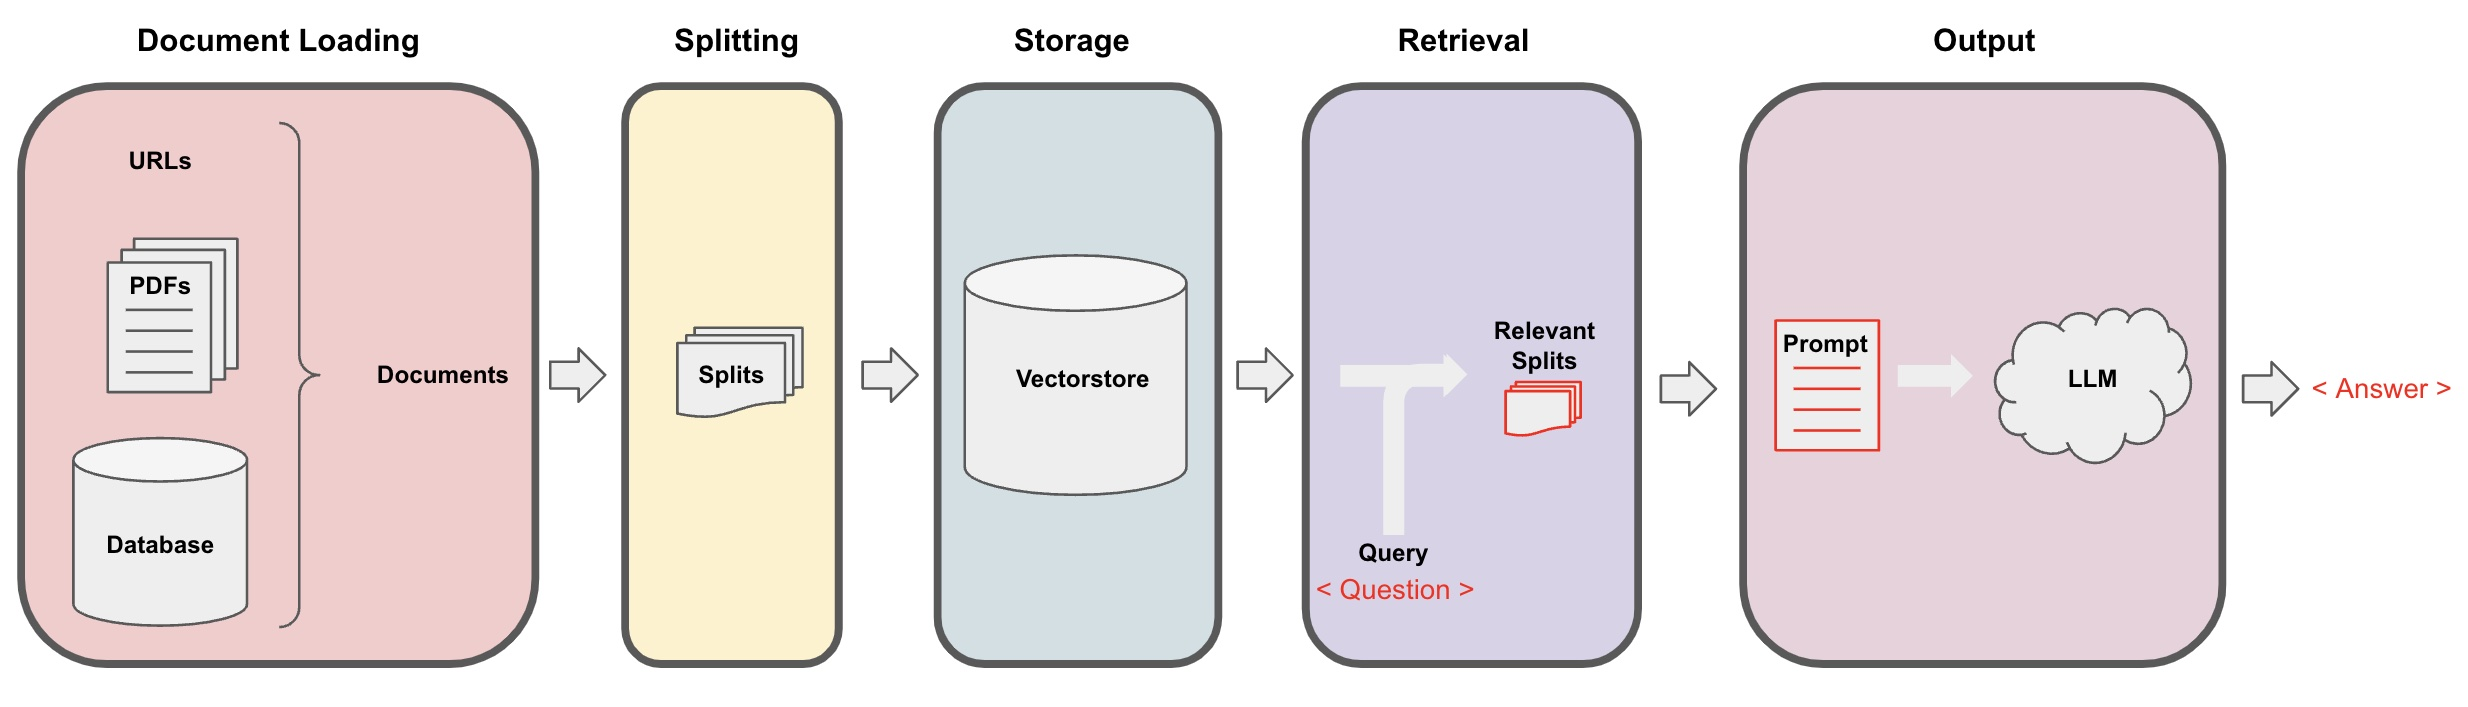
\includegraphics[height=0.18\pdfpageheight, width=0.8\pdfpagewidth]{images/QAchain.jpeg}
        \caption[QA Over Docs]{Il diagramma di flusso che descrive la catena QA Over Docs.}
        \label{fig:qaoverdocs}
    \end{figure}
\end{center}

Per il lavoro di tesi, in realtà, della catena sono state utilizzate le fasi dalla 4 in poi dato che bisognava realizzare un certo preprocessing sui dati, come aggiungere dei metadati.